\documentclass[9pt,twocolumn,twoside]{../../styles/osajnl}
\usepackage{fancyvrb}
\usepackage[utf8]{inputenc}
\usepackage{listings,lstautogobble}
\usepackage{xcolor}
\journal{i524}

\definecolor{RoyalBlue}{cmyk}{1, 0.50, 0, 0}


\title{An Overview of the Java Message Service (JMS)}


\lstset{language=Java,
    keywordstyle=\color{RoyalBlue},
    basicstyle=\scriptsize\ttfamily,
    commentstyle=\ttfamily\itshape\color{gray},
    stringstyle=\ttfamily,
    showstringspaces=false,
    breaklines=true,
    frameround=ffff,
    frame=single,
    rulecolor=\color{black},
    autogobble=true
}

\author[1]{Rahul Singh}

\affil[1]{School of Informatics and Computing, Bloomington, IN 47408, U.S.A.}

\affil[*]{Corresponding authors: rahpsing@iu.edu}

\dates{\today}

\ociscodes{Cloud, I524}

% replace this with your url in github/gitlab
\doi{\url{https://github.com/rahpsing/sp17-i524/paper1/S17-IR-2036/report.pdf}}


\begin{abstract}
Enterprise applications coordinate with each other through the
exchange of asynchronous requests termed 'messages'. Messages contain
precisely formatted data that describe specific business
actions. Through the exchange of these messages each application
tracks the progress of the enterprise. Messaging systems are expected
to support fault tolerance, load balancing, scalability, and
transactional support. JMS provides an intersection of messaging
system common to all products. The Java Message Service (JMS) provides
a standardized API for sending and receiving messages that can be used
with many different messaging systems \cite{www-jms-fischli-article}. \newline
\end{abstract}

\setboolean{displaycopyright}{true}

\begin{document}

\maketitle

\section{Introduction}

RMI(Remote Method Invocation) and RPC (Remote Procedure Call) were the
most widely used messaging systems in enterprise applications. With
the advent of distributed systems, a need arised for a loosely coupled
messaging API whose implementation wouldn't depend on knowing the
details of the receiver components unlike RMI and RPC. Sun along with
several partner companies, introduced the JMS API which defines a
common set of interfaces and associated semantics that allow programs
written in the Java programming language to communicate with other
messaging implementations. JMS is a part of the Java Platform,
Enterprise Edition, and is defined by a specification developed under
the Java Community Process as JSR 914 \cite{www-jms-javajsr}.  It is a
messaging standard that allows application components based on the
Java Enterprise Edition (Java EE) to create, send, receive, and read
messages. It allows the communication between different components of
a distributed application to be loosely coupled, reliable, and
asynchronous \cite{www-jms-oracle}. The JMS API minimizes the set of
concepts a programmer must learn in order to use messaging products
but provides enough features to support sophisticated messaging
applications.

\section{JMS API Architecture}

\begin{figure}[htbp]
\centering
\fbox{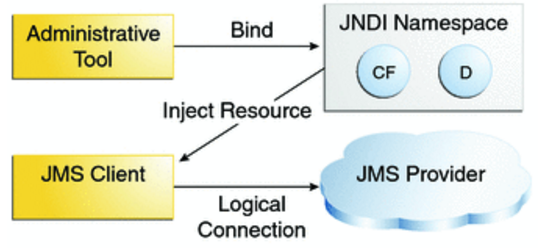
\includegraphics[width=\linewidth]{images/jmsarchitecture}}
\caption{\cite{www-jms-tutorialoracle} Jms architecture}
\label{fig:JMS Objects}
\end{figure}

A JMS application consists of the following major components.  A JMS
provider is a messaging system that implements the JMS interfaces and
provides administrative and control features. An implementation of the
Java EE platform includes a JMS provider
\cite{www-jms-tutorialoracle}. JMS Clients are the Java language
programs that send and receive messages. Any Java EE application
component can act as a JMS client.  Messages are the objects used to
communicate information between its clients.  Administered Objects are
preconfigured JMS objects created by an administrator for the use of
clients.  JMS administered objects are 'destinations' and 'connection
factories'. Destinations are the object that a client uses to specify
the destination of messages it sends and the source from where it
receives them.  A client uses a Connection Factory object to establish
connection with a provider.

Administrative tools allow a user to bind destinations and connection
factories into a JNDI (Java Naming and Directory Inteface)
namespace. A JMS client can then use resource injection to access the
administered objects in the namespace and then establish a logical
connection to the same objects through the JMS provider
\cite{www-jms-tutorialoracle}.


\section{JMS Communication Models}

Before the advent of JMS, message provider systems supported either
the point-to-point or the publish/subscribe approach to messaging
implementations. The JMS specification provides common interfaces that
enables a user to use the JMS API in a way that is not specific to
either domain. A stand-alone JMS provider can implement one or both
domains. A Java EE provider must implement both domains.

\subsection{Point-to-point model}

\begin{figure}[htbp]
\centering
\fbox{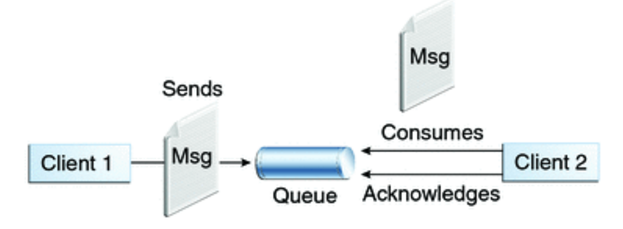
\includegraphics[width=\linewidth]{images/point-to-point}}
\caption{\cite{www-jms-tutorialoracle} Point-to-Point model}
\label{fig:Point-to-Point messaging}
\end{figure}

Point-to-point (PTP) domains are built around the concept of message
queues.  Each message is addressed to a specific queue; clients
extract messages from the queue(s) established to hold their
messages. Queues retain all messages sent to them until the messages
are consumed or expire.

\subsection{Publish/Subscribe model}

\begin{figure}[htbp]
\centering
\fbox{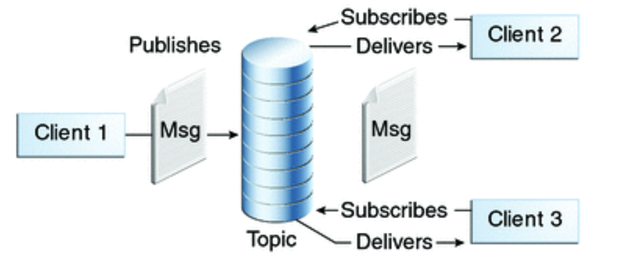
\includegraphics[width=\linewidth]{images/publish-subscribe}}
\caption{\cite{www-jms-tutorialoracle} Publish/Subscribe model}
\label{fig: Publish/Subscribe messaging}
\end{figure}

In a publish/subscribe product or application, each message can have
multiple consumers. Clients address messages to a topic, which is
equivalent to a bulletin board. Publishers and subscribers are
anonymous and can dynamically publish or subscribe to the content
hierarchy. The system shall take care of distributing the messages
arriving from a topic’s multiple publishers to its multiple
subscribers. Topics shall retain messages only for the time it takes
to distribute them to current subscribers.  Publishers and subscribers
have a timing dependency. A client that subscribes to a topic can
consume only messages published after the client has created a
subscription, and the subscriber must continue to be active in order
for it to consume messages \cite{www-jms-tutorialoracle}.


\section{JMS Programming model}

\begin{figure}[htbp]
\centering
\fbox{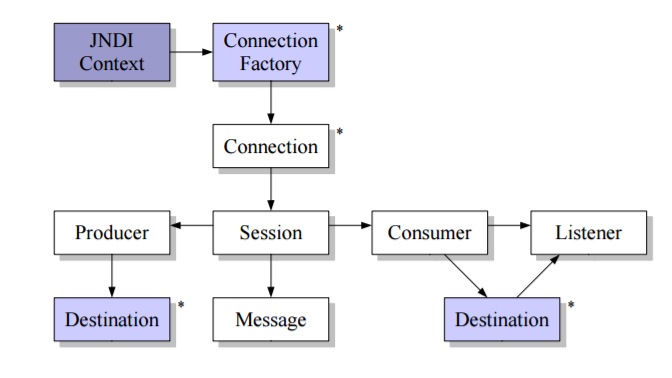
\includegraphics[width=\linewidth]{images/programming-model}}
\caption{\cite{www-jms-fischli-article} Jms programming model}
\label{fig:JMS Programming Objects}
\end{figure}

To implement the JMS specification, a series of objects shall be
created and registered to the system follows.

\subsection{Creating administered objects and binding resources}

Creating and configuring connection factories and destinations are
responsibilities of the system administrator.

\begin{lstlisting}
Properties env = new Properties();
env.put(Context.INITIAL_CONTEXT_FACTORY,
"org.exolab.jms.jndi.InitialContextFactory");
env.put(Context.PROVIDER\_URL, "tcp://localhost:3035/");
Context context = new InitialContext(env);
\end{lstlisting}

Alternatively, these administered objects shall also be created from
the server admin console available in Glassfish or any other
application servers.  A JMS client can obtain access to connection
factories and destinations by looking them up using JNDI.

\begin{lstlisting}
ConnectionFactory factory =
(ConnectionFactory)context.lookup("ConnectionFactory"); 
Destination destination = (Destination)context.lookup("Topic");
\end{lstlisting}

A connection encapsulates a virtual connection with a JMS provider
and is used to create one or more sessions.

\begin{lstlisting}
Connection connection = factory.createConnection();
connection.start();

Session session = connection.createSession(false,
Session.AUTO_ACKNOWLEDGE );
\end{lstlisting}

\subsection{Creating a message object}

The JMS API provides methods for creating messages of each type and
for filling in their contents. For example, to create and send a
TextMessage, the following syntax shall be used.

\begin{lstlisting}
TextMessage message = session.createTextMessage();
message.setText(msg_text); // msg_text is a String
\end{lstlisting}

\subsection{Creating a producer and sending the message}

A message producer is an object that is created by a session and used
for sending messages to a destination.  A Session object is used to
create a MessageProducer for a destination. A Message producer can be
created for a Destination object, a Queue object, or a Topic object.

\begin{lstlisting}
MessageProducer producer = session.createProducer(destination);
MessageProducer producer = session.createProducer(queue);
MessageProducer producer = session.createProducer(topic);
\end{lstlisting}

Once a message producer has been created, it shall be used to send
messages by using the send method.

\begin{lstlisting}
producer.send(message);
\end{lstlisting}

\subsection{Consuming a message}

A message consumer is an object that is created by a session and used
for receiving messages sent to a destination.  A message consumer
allows a JMS client to register itself in a destination with a JMS
provider. The JMS provider manages the delivery of messages from a
destination to the registered consumers of the destination.  Similar
to a producer a Message Consumer can be created for a Destination
object, a Queue object, or a Topic object.

\begin{lstlisting}
MessageConsumer consumer = session.createConsumer(destination);
MessageConsumer consumer = session.createConsumer(queue);
MessageConsumer consumer = session.createConsumer(topic);

Message m = consumer.receive();
\end{lstlisting}

To support asynchronous operations, JMS defines the concept of a
listener.  A message listener is an object that acts as an
asynchronous event handler for messages. The listener defines an
onMessage method, where we shall define the actions that need to be
taken once a message arrives.

A message listener shall be registered with a specific MessageConsumer
by using the setMessageListener method defined by the API.

\begin{lstlisting}
Listener myListener = new Listener();
consumer.setMessageListener(myListener);
\end{lstlisting}

\section{Anatomy of the JMS Message}


A JMS message carries application data and provides event
notification.  A JMS message has three parts - the message headers
provide metadata and routing information, the message properties are
defined by the JMS client, the message body carries the payload of the
message When a message is delivered, the properties and the body of
the message are made read-only \cite{www-jms-fischli-article}.

\subsection{Types Of Message}

Message types
\begin{itemize}
\item TextMessage - contains String as payload.
\item ObjectMessage - contains Java serializable object as its payload.
\item Bytes Message -contains an array of bytes as its payload.
\item Stream Message - carries stream of Java primitive types as its payload.
\item Map Message - carries a set of name-value pairs as its payload.
\end{itemize}

\section{Message acknowlegement and guaranteed delivery}


Message acknowledgment is part of the protocol between the client
runtime library of the JMS provider and the message server
\cite{www-jms-fischli-article}. The acknowledgment protocol allows the
JMS provider to guarantee delivery of messages to its
consumers/subscribers.

In the point-to-point domain messages are always guaranteed to be
delivered whereas, in the publish/subscribe domain messages are only
guaranteed to be delivered to durable subscribers.  If a consumer
fails to acknowledge a message, the server considers the message
undelivered and shall attempt to redeliver it.

JMS specifies three acknowledgment modes which are set when a session
is created:
\begin{itemize}
\item AUTO-ACKNOWLEDGE - The session automatically acknowledges
a client's receipt of a message after a successful return from the
receive() or the onMessage() method.
\item CLIENT-ACKNOWLEGE - The client
acknowledges a message by calling the message's acknowledge() method
which gives the client a finer grained control.
\item DUPS-OK-ACKNOWLEDGE - The session lazily acknowledges the
delivery of messages which may result in the delivery of duplicate
messages if the JMS provider fails \cite{www-jms-fischli-article}.

\end{itemize}


\section{Conclusion}
JMS provides a connection oriented approach to messaging in
distributed systems. It provides loosely coupled communication by
allowing objects to communicate with each other without knowing their
implementation details, thus overcoming the drawbacks of RMI. It
supports both one-to-one and many-to-many communication model and
guarantees message delivery depending on the provider implementation.


% Bibliography

\bibliography{references}


\end{document}
